\documentclass[dvipsnames, svgnames, x11names, a4paper, 11pt]{article}

% URLs and hyperlinks ------------------------------
\usepackage{hyperref}
\hypersetup{
    colorlinks=true,
    linkcolor=NavyBlue,
    filecolor=magenta,      
    urlcolor=blue,
}
\usepackage{xurl}
%---------------------------------------------------

\usepackage{float}
\usepackage{graphicx}
\usepackage{listings}
\usepackage{color}
\usepackage{xcolor}

\definecolor{dkgreen}{rgb}{0,0.6,0}
\definecolor{gray}{rgb}{0.5,0.5,0.5}
\definecolor{mauve}{rgb}{0.58,0,0.82}

\lstset{frame=tb,
    language=vhdl,
    aboveskip=3mm,
    belowskip=3mm,
    showstringspaces=false,
    columns=flexible,
    basicstyle=\ttfamily,
    numbers=left,
    numberstyle=\small\color{gray},
    keywordstyle=\bfseries\color{Green4},
    commentstyle=\color{gray},
    stringstyle=\color{mauve},
    breaklines=true,
    breakatwhitespace=true,
    tabsize=4,
    identifierstyle=\color{black}
}

\usepackage{xepersian}
\settextfont{Yas}

\title{حافظه‌های \lr{ROM} و \lr{BRAM}}
\author{مهدی حق‌وردی}

\begin{document}
\maketitle
\tableofcontents

\section{توضیحات فایل‌های تمرین}
\subsection{فایل \lr{\texttt{rom8x8}}}
این فایل، ساده‌ترین فایل این تمرین است که شامل یک موجودیت به نام
\lr{\texttt{rom8x8}}
و یک معماری به نام 
\lr{\texttt{behave}}
است.

\subsubsection{توضیحات موجودیت \lr{\texttt{rom8x8}}}
این موجودیت شامل دو پورت است:
\begin{itemize}
\item 
\lr{\texttt{addr}}

این پورت یک ورودی 
\lr{\texttt{std\_logic\_vector}} 
۳ بیتی است که در واقع مقدار خروجی را تعیین می‌کند.

\item 
\lr{\texttt{dout}}

این پورت هم یک پورت خروجی از نوع 
\lr{\texttt{std\_logic\_vector}}
۷ بیتی است که مقدار خروجی روی آن قرار می‌گیرد.
\end{itemize}

\subsubsection{توضیحات معماری \lr{\texttt{behave}}}
این تنها معماری حاضر برای موجودیت 
\lr{\texttt{rom8x8}}
است که در واقع یک \lr{decoder} ۳ به ۸ است.

مقادیری که برای خروجی انتخاب شده‌اند کاملا \lr{hard code} شده‌اند و این کاملا با نام موجودیت (که \lr{\texttt{rom}} است) هماهنگی دارد.

در معماری از 
\lr{language feature}
عی به نام 
\lr{\texttt{with ... select}}
استفاده شده است که با توجه به مقدار 
\lr{\texttt{addr}}
خروجی را روی 
\lr{\texttt{dout}}
قرار می‌دهد.

\subsection{فایل \lr{romram}}
این فایل در واقع کل پروژه و کد این شکل است:
\begin{figure}[H]
\begin{center}
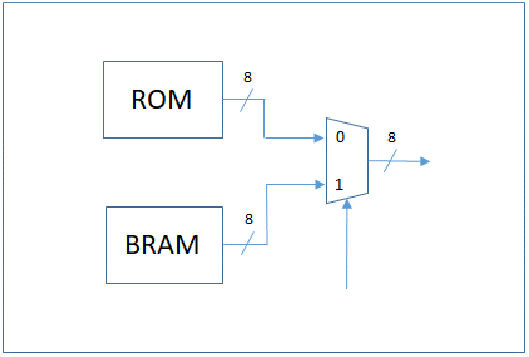
\includegraphics[width=0.7\textwidth, height=0.3\textheight]{images/project}
\end{center}
\end{figure}
چرا کد این شکل است؟

چون در کد مشاهده‌ می‌شود که مشخصا موجودیت‌های 
\lr{\texttt{rom8x8}}
،
\lr{\texttt{clock\_divide}}
و
\lr{\texttt{bram8x8}}
در آن به عنوان یک 
\lr{component}
استفاده شده‌اند (که موجودیت‌هایی هستند که در شکل وجود دارند، البته مالتی پلکسری که در شکل است در قسمت معماری همین فایل تعریف شده است).

کد شامل یک موجودیت به نام
\lr{\texttt{romram}}
و یک معماری به نام
\lr{\texttt{structural}}
است.

\subsubsection{موجودیت \lr{\texttt{romram}}}
موجودیت دارای دو ورودی و یک خروجی‌ست
\begin{itemize}
\item 
ورودی‌ها

\begin{itemize}
\item \lr{\texttt{clk\_100MHZ}}

\item  \lr{\texttt{switch}}
\end{itemize}

\item 
خروجی
\begin{itemize}
\item \lr{\texttt{leds}}
\end{itemize}

\end{itemize}
\subsubsection{معماری \lr{\texttt{structural}}}

\subsection{فایل \lr{clockDevider}}

\end{document}